\documentclass[tikz]{standalone}
\usepackage{amsmath}
\usepackage{amssymb}
\begin{document}
	
	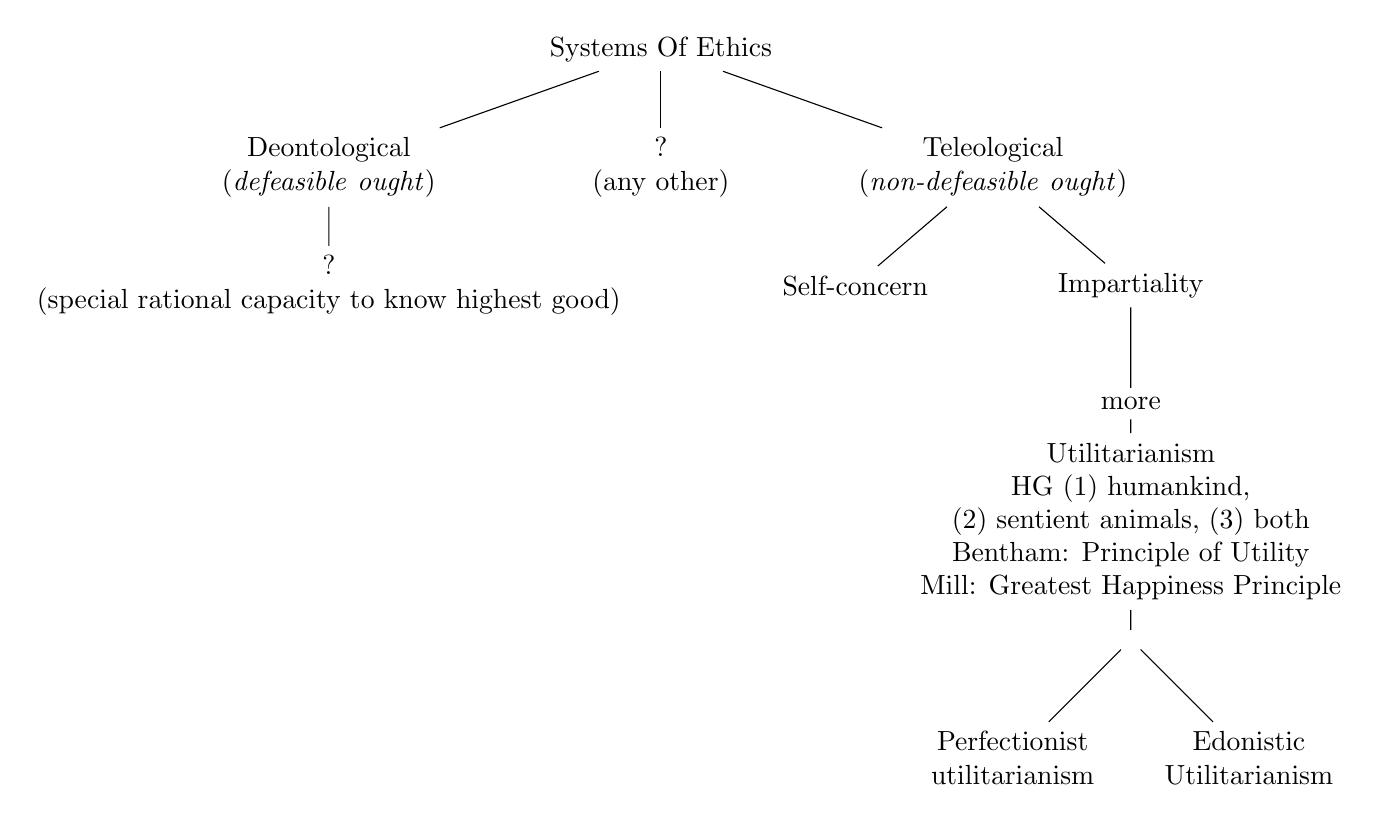
\begin{tikzpicture}[every node/.style={align=center},level 1/.style={sibling distance=12em},level 2/.style={sibling distance=35mm}, level 3/.style={sibling distance=30mm}, level 4/.style={sibling distance=30mm}]
		\node {Systems Of Ethics}
		[sibling distance=6cm]
		child { node {Deontological \\ (\textit{defeasible} \textit{ought})} 
			child { node {? \\ (special rational capacity to know highest good)}}} % <- End Deontological
		child { node [draw=none] {? \\ (any other)} }
		child { node {Teleological \\ (\textit{non-defeasible} \textit{ought})} child {node {Self-concern}} child {node {Impartiality} child {node {more} child {node {Utilitarianism \\ HG (1) humankind, \\ (2) sentient animals, (3) both \\ Bentham: Principle of Utility \\ Mill: Greatest Happiness Principle}
						child {node [] {} 
							child {node {Perfectionist \\ utilitarianism} }
							child {node {Edonistic \\ Utilitarianism}}}} }}}
		;
	\end{tikzpicture}
	
\end{document}
